\usepackage{ifthen}

% Define an agenda item
%
% Arguments:
% 1: Identifier of the agenda item, should be all lower-case
% 2: Type of the agenda item: lecture or lab
% 3: English title of the agenda item
% 4: English full description of the agenda item
% 5: French title of the agenda item
% 6: French full description of the agenda item
\newcommand\defagendaitem[6]{
  \ifthenelse{\equal{\agendalanguage}{french}}{
    \expandafter\def\csname #1@#2@title\endcsname {#5}
    \expandafter\def\csname #1@#2@contents\endcsname {#6}
  }{
    \expandafter\def\csname #1@#2@title\endcsname {#3}
    \expandafter\def\csname #1@#2@contents\endcsname {#4}
  }
}

% Show/render an agenda item
%
% Arguments:
% 1: Identifier of the agenda item, as defined by \defagendaitem
% 2: Type of the agenda item: lecture or lab
\newcommand\showagendaitem[2]{%
  \ifthenelse{\boolean{hlineneeded}}{\\\hline}{\setboolean{hlineneeded}{true}}%
    \ifthenelse{\equal{\agendalanguage}{french}}{%
      \ifthenelse{\equal{#2}{lecture}}%
      {Cours &}%
      {%
        \ifthenelse{\equal{#2}{lab}}{%
          \ifthenelse{\equal{\trainingtype}{online}}{Démo &}{TP &}%
        }%
        {}%
      }%
    }{%
      \ifthenelse{\equal{#2}{lecture}}%
      {Lecture &}%
      {%
        \ifthenelse{\equal{#2}{lab}}{%
          \ifthenelse{\equal{\trainingtype}{online}}{Demo &}{Lab &}%
        }%
        {}%
      }%
    }%
    \csname #1@#2@title\endcsname &%
    \vspace{-12pt}%
    \csname #1@#2@contents\endcsname%
}%

% Define a board
%
% Arguments:
% 1: Identifier for the board, must be all lower-case
% 2: English title
% 3: English full description
% 4: French title
% 5: French full description
% 6: Board picture
\newcommand\defboard[6]{
  \ifthenelse{\equal{\agendalanguage}{french}}{
    \expandafter\def\csname #1@title\endcsname {#4}
    \expandafter\def\csname #1@contents\endcsname {#5}
  }{
    \expandafter\def\csname #1@title\endcsname {#2}
    \expandafter\def\csname #1@contents\endcsname {#3}
  }
  \expandafter\def\csname #1@image\endcsname {#6}
}

% Show/render a board
%
% Arguments:
% 1: Identifier of the board, as defined by \defboard
\newcommand\showboarditem[1]{
  \begin{tabularx}{\textwidth}{p{7cm}p{11cm}}
    \arrayrulecolor{blorange}
    \hline
    \multicolumn{1}{l}{\textbf{\textcolor{blorange}{\large \csname #1@title\endcsname}}} & \\
    \hline
    \arrayrulecolor{gray}
    \csname #1@contents\endcsname &
    \csname #1@image\endcsname \\
  \end{tabularx}
}

% Start an agenda by finding
% out if it is a morning or an
% afternoon if the training
% takes place on site
%
% Arguments:
% 1: Number of the half-day
\newcommand\showagendaday[1]{%
  \arrayrulecolor{blorange}%
  \\\hline%
  \multicolumn{3}{l}{%
    \textbf{\textcolor{blorange}{\large%
      \ifthenelse{\equal{\trainingtype}{online}}{%
        \showonlineagendaday{#1}%
      }{%
        \pgfmathparse{int(mod(#1, 2))}%
        \ifnum\pgfmathresult=1%
          \pgfmathparse{int((#1 + 1) / 2)}%
          \showonsiteagendaday{\pgfmathresult}{morning}%
        \else%
          \pgfmathparse{int(#1 / 2)}%
          \showonsiteagendaday{\pgfmathresult}{afternoon}%
        \fi%
      }%
    }}%
  } \\%
  \hline%
  \setboolean{hlineneeded}{false}%
  \arrayrulecolor{gray}%
}%

% Start an online agenda half-day
%
% Arguments:
% 1: Number of the half-day
\newcommand\showonlineagendaday[1]{%
  \ifthenelse{\equal{\agendalanguage}{french}}{%
    Demi-journée #1%
  }{%
    Half day #1%
  }%
}%

% Start an on-site agenda half-day
%
% Arguments:
% 1: Number of the day
% 2: "morning" or "afternoon"
\newcommand\showonsiteagendaday[2]{%
  \ifthenelse{\equal{\agendalanguage}{french}}{%
    \ifthenelse{\equal{#2}{morning}}{%
      Jour #1 - Matin%
    }{%
      Jour #1 - Après-midi%
    }%
  }{%
    \ifthenelse{\equal{#2}{morning}}{%
      Day #1 - Morning%
    }{%
      Day #1 - Afternoon%
    }%
  }%
}%

\defboard
{stm32mp1}
{STM32MP1 Discovery Kit}
{
  One of these Discovery Kits from STMicroelectronics: {\bf
  STM32MP157A-DK1}, {\bf STM32MP157D-DK1}, {\bf STM32MP157C-DK2} or
  {\bf STM32MP157F-DK2}
  \begin{itemize}
  \item STM32MP157, dual Cortex-A7 processor from STMicroelectronics
  \item USB powered
  \item 512 MB DDR3L RAM
  \item Gigabit Ethernet port
  \item 4 USB 2.0 host ports
  \item 1 USB-C OTG port
  \item 1 Micro SD slot
  \item On-board ST-LINK/V2-1 debugger
  \item Arduino compatible headers
  \item Audio codec, buttons, LEDs
  \item LCD touchscreen (DK2 kits only)
  \vspace{-0.7cm}
  \end{itemize}
}
{Plateforme STM32MP1}
{
  Une de ces cartes de STMicroelectronics : {\bf
  STM32MP157A-DK1}, {\bf STM32MP157D-DK1}, {\bf STM32MP157C-DK2} ou
  {\bf STM32MP157F-DK2}
  \begin{itemize}
  \item Processeur STM32MP157, double Cortex-A7, de STMicroelectronics
  \item Alimentée par USB
  \item 512 Mo DDR3L RAM
  \item Port Gigabit Ethernet port
  \item 4 ports hôte USB 2.0
  \item 1 port USB-C OTG
  \item 1 connecteur Micro SD
  \item Debugger ST-LINK/V2-1 sur la carte
  \item Connecteurs compatibles Arduino Uno v3
  \item Codec audio
  \item Divers : boutons, LEDs
  \item Écran LCD tactile (uniquement sur cartes DK2)
  \vspace{-0.7cm}
  \end{itemize}
}
{
  \begin{center}
    \includegraphics[width=5cm]{../slides/discovery-board-dk1/discovery-board-dk1.png}
  \end{center}
}

\defagendaitem
{qna}
{misc}
{Questions and Answers}
{
  \begin{itemize}
  \item Questions and answers with the audience about the course topics
  \item Extra presentations if time is left, according what most
        participants are interested in.
  \end{itemize}
}
{Questions / réponses}
{
  \begin{itemize}
  \item Questions et réponses avec les participants à propos des sujets abordés.
  \item Présentations supplémentaires s'il reste du temps, en fonction des demandes
        de la majorité des participants.
  \end{itemize}
}


\defboard
{beagleboneblack}
{BeagleBone Black}
{
  {\bf BeagleBone Black} or {\bf BeagleBone Black Wireless} board
  \begin{itemize}
  \item An ARM AM335x (single Cortex-A8) processor from Texas
    Instruments
  \item USB powered
  \item 512 MB of RAM
  \item 2 or 4 GB of on-board eMMC storage
  \item USB host and device
  \item HDMI output
  \item 2 x 46 pins headers, to access UARTs, SPI buses, I2C buses
    and more.
  \item Ethernet or WiFi
  \end{itemize}
  \vspace{-0.7cm}
}
{BeagleBone Black}
{
  Carte {\bf BeagleBone Black} ou {\bf BeagleBone Black Wireless}
  \begin{itemize}
  \item Un processeur ARM AM335x de Texas Instruments (à base de
    Cortex-A8), avec accélération 3D, etc.
  \item 512 Mo de RAM
  \item 2 ou 4 Go de stockage eMMC
  \item USB hôte et device
  \item Sortie HDMI
  \item Connecteurs à 2 x 46 broches, pour accéder aux UARTs, aux bus
    SPI, aux bus I2C, et à d'autres entrées/sorties du processeur.
  \item Ethernet ou WiFi
  \vspace{-0.7cm}
  \end{itemize}
}
{
  \begin{center}
    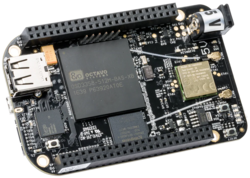
\includegraphics[width=5cm]{../slides/beagleboneblack-board/beagleboneblack_sd.png}
  \end{center}
}

\defboard
{beagleplay}
{BeaglePlay}
{
  {\bf BeaglePlay} board
  \begin{itemize}
    \item Texas Instruments AM625x (4xARM Cortex-A53 CPU)
    \item SoC with 3D acceleration, integrated MCU and many other peripherals.
    \item 2 GB of RAM
    \item 16 GB of on-board eMMC storage
    \item USB host and USB device, microSD, HDMI
    \item 2.4 and 5 GHz WiFi, Bluetooth and also Ethernet
    \item 1 MicroBus Header (SPI, I2C, UART, ...), OLDI and CSI connector.
  \vspace{-0.7cm}
  \end{itemize}
}
{BeaglePlay}
{
  Carte {\bf BeaglePlay}
  \begin{itemize}
    \item SoC Texas Instruments AM625x (CPU 4xARM Cortex-A53)
    \item SoC avec accélération 3D, MCU intégré et de nombreux autres périphériques.
    \item 2 GB de RAM
    \item 16 Go de stockage eMMC
    \item USB hôte et device, microSD, HDMI
    \item WiFi 2.4 and 5 GHz, Bluetooth et aussi Ethernet
    \item 1 Header MicroBus (SPI, I2C, UART, ...), connecteurs OLDI et CSI.
  \vspace{-0.7cm}
  \end{itemize}
}
{
  \begin{center}
    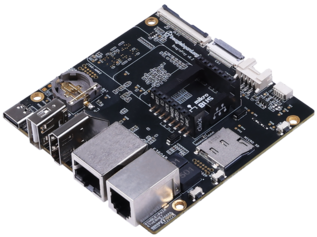
\includegraphics[width=5cm]{../slides/beagleplay-board/beagleplay_sd.png}
  \end{center}
}

\defboard
{espressobin}
{Hardware platform for practical labs}
{
  {\bf Globalscale EspressoBin} board
  \begin{itemize}
  \item Dual Cortex A53 Marvell Armada 3720 SoC
  \item Onboard switch with 2x 1Gbps interfaces
  \item Extra 1Gbps interface
  \item 1GB RAM
  \item 1x SATA interface
  \item 1x USB 3.0 interface
  \end{itemize}
}
{Plateforme matérielle pour les travaux pratiques}
{
  Carte {\bf Globalscale EspressoBin}
  \begin{itemize}
  \item SoC Marvell Armada 3720 SoC (CPU 2xARM Cortex A53)
  \item Switch Ethernet avec 2 interfaces Gigabit
  \item Interface Gigabit Ethernet additionnelle
  \item 1GB de RAM
  \item 1x interface SATA
  \item 1x interface USB 3.0
  \end{itemize}
}
{
  \begin{center}
    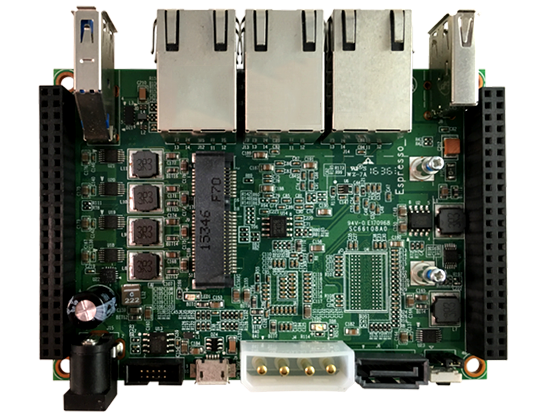
\includegraphics[width=5cm]{../slides/espressobin/espressobin.png}
  \end{center}
}


\def \training{debugging}

% Title
\ifthenelse{\equal{\agendalanguage}{french}}{
  \def \trainingtitle{Formation debugging, profiling, tracing et analyse de performance sous Linux}
}{
  \def \trainingtitle{Linux debugging, profiling, tracing and performance analysis training}
}

% Duration
\ifthenelse{\equal{\trainingtype}{online}}{
  \def \trainingduration{4}
}{
  \def \trainingduration{3}
}

% Training objectives
\ifthenelse{\equal{\agendalanguage}{french}}{
  \def \traininggoals{
    \begin{itemize}
    \item Être capable de comprendre les principaux concepts de Linux
      qui sont liés à l'analyse de performance: processus, threads,
      gestion de la mémoire, mémoire virtuelle, contextes d'exécution,
      etc.
    \item Être capable d'analyser pourquoi un système est chargé et
      quels sont les éléments qui contribuent à cette charge avec les
      outils usuels d'observabilité sous Linux.
    \item Être capable de débugger une application espace utilisateur
      avec {\em gdb}, soit en direct soit {\em post-mortem} suite à un
      crash, et analyser le contenu de binaires ELF.
    \item Être capable d'utiliser le {\em tracing} et le {\em profiling}
      sur une application espace utilisateur et comprendre ses
      interactions avec le noyau Linux afin de corriger des bugs, en
      utilisant {\em strace}, {\em ltrace}, {\em perf} ou {\em
        Callgrind}
    \item Être capable d'utiliser le {\em tracing} et le {\em profiling}
      le système Linux complet, en utilisant {\em perf}, {\em ftrace},
      {\em kprobe}, les outils {\em eBPF}, {\em kernelshark} ou {\em
        LTTng}
    \item Être capable de débugger des problèmes au niveau du noyau
      Linux: debug de crash en direct ou post-mortem, analyse de
      problèmes mémoire au niveau noyau, analyse de problèmes de locks,
      utilisation de debuggers au niveau noyau.
    \end{itemize}
  }
}{
  \def \traininggoals{
    \begin{itemize}
      \vspace{-0.5cm}
    \item Be able to understand the main concepts of Linux that are
      relevant for performance analysis: process, threads, memory
      management, virtual memory, execution contexts, etc.
    \item Be able to analyze why a system is loaded and what are the
      elements that contributes to this load using common Linux
      observability tools.
    \item Be able to debug an userspace application using {\em gdb},
      either live or after a crash, and analyze the contents of ELF
      binaries.
    \item Be able to trace and profile a complete userspace application
      and its interactions with the Linux kernel in order to fix bugs
      using {\em strace}, {\em ltrace}, {\em perf} or {\em Callgrind}.
    \item Be able to understand classical memory issues and analyze them
      using {\em valgrind}, {\em libefence} or {\em Massif}.
    \item Be able to trace and profile the entire Linux system, using
      {\em perf}, {\em ftrace}, {\em kprobes}, {\em eBPF} tools, {\em
        kernelshark} or {\em LTTng}
    \item Be able to debug Linux kernel issues: debug kernel crashes
      live or post-mortem, analyze memory issues at the kernel level,
      analyze locking issues, use kernel-level debuggers.
      \vspace{-0.5cm}
    \end{itemize}
  }
}

% Training prerequisites
\def \trainingprerequisites{
  \begin{itemize}
    \prerequisitecommandline
    \prerequisiteembeddedlinux
    \prerequisiteenglish
  \end{itemize}
}

% Training audience
\ifthenelse{\equal{\agendalanguage}{french}}{
  \def \trainingaudience{
    Sociétés et ingénieurs intéressés dans le debug, profiling et
    tracing de systèmes et d'applications Linux, afin d'analyser et
    résoudre des problèmes de performance ou de latence.
  }
}{
  \def \trainingaudience{
    Companies and engineers interested in debugging, profiling and
    tracing Linux systems and applications, to analyze and address
    performance or latency problems.
  }
}

% Time ratio
\def \onsitelecturetimeratio{40}
\def \onsitelabtimeratio{60}

% Agenda items

\defagendaitem
{appstack}
{lecture}
{Linux application stack}
{
  \begin{itemize}
  \item Global picture: understanding the general architecture of a
        Linux system, overview of the major components.
  \item What is the difference between a process and a thread, how
    applications run concurrently.
  \item ELF files and associated analysis tools.
  \item Userspace application memory layout (heap, stack, shared
    libraries mappings, etc).
  \item MMU and memory management: physical/virtual address spaces.
  \item Kernel context switching and scheduling
  \item Kernel execution contexts: kernel threads, workqueues,
    interrupt, threaded interrupts, softirq
  \end{itemize}
}
{Pile logicielle Linux}
{
  \begin{itemize}
  \item Vue d'ensemble : comprendre l'architecture général d'un système
    Linux, aperçu des principaux composants
  \item Différence entre un processus et un thread, comment les
    applications fonctionnent de façon concurrente.
  \item Fichiers ELF et outils d'analyse associés.
  \item Organisation de l'espace d'adressage des applications : heap,
    stack, bibliothèques partagées, etc.
  \item MMU et gestion mémoire : espaces d'adressage physique et
    virtuel
  \item Contexte d'exécution dans le noyau : threads noyau, workqueues,
    interruptions, interruptions threadées, softirq
  \end{itemize}
}
\defagendaitem
{commontools}
{lecture}
{Common analysis \& observability tools}
{
  \begin{itemize}
  \item Analyzing an ELF file with GNU binary utilities
    ({\em objdump}, {\em addr2line}).
  \item Tools to monitor a Linux system: processes, memory
    usage and mapping, resources.
  \item Using {\em vmstat}, {\em iostat}, {\em ps}, {\em top}, {\em
      iotop}, {\em free} and understanding the metrics they provide.
  \item Pseudo filesystems: {\em procfs}, {\em sysfs} and {\em
      debugfs}.
  \end{itemize}
}
{Outils usuels d'analyse et d'observation}
{
  \begin{itemize}
  \item Analyse d'un binaire ELF avec les outils GNU ({\em objdump},
    {\em addr2line})
  \item Outils pour monitorer un système Linux : processus,
    consommation et mapping mémoire, ressources
  \item Utilisation de {\em vmstat}, {\em iostat}, {\em ps}, {\em
      top}, {\em iotop}, {\em free} et compréhension des métriques
    qu'ils fournissent.
  \item Systèmes de fichiers virtuels : {\em procfs}, {\em sysfs} et
    {\em debugfs}
  \end{itemize}
}
\defagendaitem
{checksystem}
{lab}
{Check what is running on a system and its load}
{
  \begin{itemize}
  \item Observe running processes using {\em ps} and {\em top}.
  \item Check memory allocation and mapping with {\em procfs} and {\em
      pmap}.
  \item Monitor other resources usage using {\em iostat}, {\em vmstat}
    and {\em netstat}.
  \end{itemize}
}
{Comprendre ce qui fonctionne sur un système et sa charge}
{
  \begin{itemize}
  \item Observation des processus en cours d'exécution avec {\em ps} et {\em top}
  \item Observation des mappings mémoire avec {\em procfs} et {\em pmap}
  \item Monitoring d'aurtres ressources avec {\em iostat}, {\em
      vmstat} et {\em netstat}
 \end{itemize}
}
\defagendaitem
{debugapp}
{lecture}
{Debugging an application}
{
  \begin{itemize}
  \item Using {\em gdb} on a live process.
  \item Understanding compiler optimizations impact on debuggability.
  \item Postmortem diagnostic using core files.
  \item Remote debugging with {\em gdbserver}.
  \item Extending {\em gdb} capabilities using python scripting
  \end{itemize}
}
{Debug d'une application}
{
  \begin{itemize}
  \item Utilisation de {\em gdb} sur un processus en cours d'exécution.
  \item Comprendre l'impact des optimisations du compilateur sur la
    capacité à débugger un programme.
  \item Analyse post-mortem avec des fichiers {\em core}
  \item Debug à distance avec {\em gdbserver}.
  \item Étendre les capacités de {\em gdb} en utilisant des scripts
    Python.
  \end{itemize}
}
\defagendaitem
{solvecrash}
{lab}
{Solving an application crash}
{
  \begin{itemize}
  \item Analysis of compiled C code with compiler-explorer to understand
    optimizations.
  \item Managing {\em gdb} from the command line, then from an IDE.
  \item Using {\em gdb} Python scripting capabilities.
  \item Debugging a crashed application using a coredump with {\em gdb}.
  \end{itemize}
}
{Résoudre un crash applicatif}
{
  \begin{itemize}
  \item Analyse d'un code C compilé avec \code{compiler-explorer} pour
    comprendre les optimisations.
  \item Utilisation de {\em gdb} en ligne de commande, puis depuis un
    IDE.
  \item Utilisation des possibilités de scripting Python dans {\em gdb}.
  \item Debugger une application {\em post mortem} avec un {\em core
      dump} et {\em gdb}
  \end{itemize}
}
\defagendaitem
{tracing}
{lecture}
{Tracing an application}
{
  \begin{itemize}
  \item Tracing system calls with {\em strace}.
  \item Tracing library calls with {\em ltrace}.
  \item Overloading library functions using {\em LD\_PRELOAD}.
  \end{itemize}
}
{Tracing d'une application}
{
  \begin{itemize}
  \item Tracing des appels systèmes avec {\em strace}.
  \item Tracing des appels à des bibliothèques partagées avec {\em ltrace}.
  \end{itemize}
}
\defagendaitem
{debugappissue}
{lab}
{Debugging application issues}
{
  \begin{itemize}
  \item Analyze dynamic library calls from an application using
    {\em ltrace}.
  \item Overloading library functions using {\em LD\_PRELOAD}.
  \item Analyzing an application system calls using {\em strace}.
  \end{itemize}
}
{Débugger des problèmes applicatifs}
{
  \begin{itemize}
  \item Analyser les appels à des bibliothèques partagées d'une
    application en utilisant {\em ltrace}.
  \item Débugger une application qui fonctionne de manière incorrecte
    en utilisant {\em strace}.
  \end{itemize}
}
\defagendaitem
{memory}
{lecture}
{Memory issues}
{
  \begin{itemize}
  \item Usual memory issues: buffer overflow, segmentation fault,
    memory leaks, heap-stack collision.
  \item Memory corruption tooling, {\em valgrind}, {\em libefence},
    etc.
  \item Heap profiling using {\em Massif} and {\em heaptrack}
  \end{itemize}
}
{Problèmes liés à la mémoire}
{
  \begin{itemize}
  \item Problèmes classiques liés à la mémoire : {\em buffer overflow},
    {\em segmentation fault}, fuite mémoire, collision pile/tas.
  \item Outils de détection/investigation de problèmes mémoires : {\em
      valgrind}, {\em libefence}, etc.
  \item Profiling de l'utilisation du tas en utilisant {\em Massif}
  \end{itemize}
}
\defagendaitem
{memory}
{lab}
{Debugging memory issues}
{
  \begin{itemize}
  \item Memory leak and misbehavior detection with {\em valgrind} and
    {\em vgdb}.
  \item Visualizing application heap using {\em Massif}.
  \end{itemize}
}
{Débugger des problèmes liés à la mémoire}
{
  \begin{itemize}
  \item Fuites mémoire et détection de comportement incorrects avec
    {\em valgrind} et {\em vgdb}.
  \item Problèmes de performance liés à une sur-allocation.
  \item Visualisation de l'utilisation du tas par une application en
    utilisant {\em Massif}.
  \end{itemize}
}
\defagendaitem
{appprofile}
{lecture}
{Application profiling}
{
  \begin{itemize}
  \item Performances issues.
  \item Gathering profiling data with {\em perf}.
  \item Analyzing an application callgraph using {\em Callgrind}
    and {\em KCachegrind}.
  \item Interpreting the data recorded by {\em perf}.
  \end{itemize}
}
{Profiling d'application}
{
  \begin{itemize}
  \item Problèmes de performance.
  \item Récupération d'informations de profiling avec {\em perf}.
  \item Analyse du graphe d'appel d'une application avec {\em
      Callgrind} et {\em KCachegrind}.
  \item Filtrage du jeu de données récupéré.
  \item Interprétation, des données enregistrées avec {\em perf}.
  \end{itemize}
}
\defagendaitem
{appprofile}
{lab}
{Application profiling}
{
  \begin{itemize}
  \item Profiling an application with {\em Callgrind}/{\em
      KCachegrind}.
  \item Analyzing application performance with {\em perf}.
  \item Generating a flamegraph using {\em FlameGraph}.
  \end{itemize}
}
{Profiling d'application}
{
  \begin{itemize}
  \item Profiling d'une application avec {\em Callgrind}/{\em
      KCachegrind}.
  \item Analyse des performances d'une application avec {\em perf}.
  \item Générer un {\em flamegraph} avec {\em FlameGraph}.
  \end{itemize}
}
\defagendaitem
{profiling}
{lecture}
{System wide profiling and tracing}
{
  \begin{itemize}
  \item System wide profiling using {\em perf}.
  \item Using {\em kprobes} to hook on kernel code without
    recompiling.
    \item Application and kernel tracing and visualization using {\em
        ftrace}, {\em kernelshark} or {\em LTTng}
  \item Tracing with {\em eBPF}: core principles, usage with BCC and with libbpf
  \end{itemize}
}
{Profiling et tracing de l'ensemble du système}
{
  \begin{itemize}
  \item Profiling du système complet avec {\em perf}.
  \item Utilisation de {\em kprobes} pour ajouter des points de trace
    supplémentaires sans recompilation
    \item Tracing d'application et du noyau et visualisation des traces
      avec {\em ftrace}, {\em kernelshark} ou {\em LTTng}
  \item Tracing avec eBPF: principes généraux, développements d'outils avec BCC
  puis libbpf
  \end{itemize}
}
\defagendaitem
{profiling}
{lab}
{System wide profiling and tracing}
{
  \begin{itemize}
  \item System profiling with {\em perf}.
  \item System wide latencies debugging using {\em ftrace} and {\em
  kernelshark}.
  \end{itemize}
}
{Profiling et tracing de l'ensemble du système}
{
  \begin{itemize}
  \item Profiling du système complet avec {\em perf}.
  \item Analyse de latences système avec {\em ftrace} et {\em kernelshark}.
  \end{itemize}
}
\defagendaitem
{ebpf}
{lab}
{Tracing tool with eBPF}
{
  \begin{itemize}
  \item Python scripting with{\em bcc}.
  \item Custom tool development with libbpf.
  \end{itemize}
}
{Développement d'outils en eBPF}
{
  \begin{itemize}
  \item Scripting python avec {\em BCC}.
  \item Développement d'un outil personnalisé de tracing avec libbpf.
  \end{itemize}
}
\defagendaitem
{kernel}
{lecture}
{Kernel debugging}
{
  \begin{itemize}
  \item Kernel compilation results (\code{vmlinux}, \code{System.map}).
  \item Understanding and configuring kernel {\em oops} behavior.
  \item Post mortem analysis using kernel crash dump with {\em crash}.
  \item Memory issues ({\em KASAN}, {\em UBSAN}, {\em Kmemleak}).
  \item Debugging the kernel using {\em KGDB} and {\em KDB}.
  \item Kernel locking debug configuration options (lockdep).
  \item Other kernel configuration options that are useful for debug.
  \end{itemize}
}
{Debugging du noyau Linux}
{
  \begin{itemize}
  \item Sorties de la compilation du noyau Linux utiles pour le
    debugging (\code{vmlinux}, \code{System.map}).
  \item Comprendre et configurer le comportement des {\em kernel oops}.
  \item Analyse post-mortem d'un crash kernel avec {\em crash}.
  \item Problèmes mémoire au niveau kernel ({\em KASAN}, {\em UBSAN}, {\em Kmemleak}).
  \item Debugging du noyau Linux avec {\em KGDB} et {\em KDB}.
  \item Options du noyau Linux pour le debug des problèmes de verrous
    (lockdep)
  \item Autres options de configuration du noyau Linux utiles pour le
    debug.
  \end{itemize}
}
\defagendaitem
{kernel}
{lab}
{Kernel debugging}
{
  \begin{itemize}
  \item Analyzing an {\em oops} after using a faulty module with
    {\em obdjump} and {\em addr2line}.
  \item Debugging a deadlock problem using {\em PROVE\_LOCKING} options.
  \item Detecting undefined behavior with {\em UBSAN} in kernel code.
  \item Find a module memory leak using {\em kmemleak}.
  \item Debugging a module with {\em KGDB}.
  \end{itemize}
}
{Debugging du noyau Linux}
{
  \begin{itemize}
  \item Analyse d'un {\em oops} après utilisation d'un module noyau
    incorrect, avec {\em obdjump} et {\em addr2line}.
  \item Debugging d'un {\em deadlock} avec les options {\em PROVE\_LOCKING}.
  \item Détecter un {\em undefined behavior} avec {\em UBSAN} dans le noyau Linux.
  \item Trouver une fuite mémoire avec {\em kmemleak}.
  \item Débugger un module noyau avec {\em KGDB}.
  \end{itemize}
}

\def \onsiteagenda {
  \showagendaday{1}
  \showagendaitem{appstack}{lecture}
  \showagendaitem{commontools}{lecture}
  \showagendaday{2}
  \showagendaitem{checksystem}{lab}
  \showagendaitem{debugapp}{lecture}
  \showagendaitem{solvecrash}{lab}
  \showagendaday{3}
  \showagendaitem{tracing}{lecture}
  \showagendaitem{debugappissue}{lab}
  \showagendaitem{memory}{lecture}
  \showagendaitem{memory}{lab}
  \showagendaday{4}
  \showagendaitem{appprofile}{lecture}
  \showagendaitem{appprofile}{lab}
  \showagendaday{5}
  \showagendaitem{profiling}{lecture}
  \showagendaitem{profiling}{lab}
  \showagendaitem{ebpf}{lab}
  \showagendaday{6}
  \showagendaitem{kernel}{lecture}
  \showagendaitem{kernel}{lab}
}

\def \onlineagenda {
  \showagendaday{1}
  \showagendaitem{appstack}{lecture}
  \showagendaitem{commontools}{lecture}
  \showagendaitem{checksystem}{lab}
  \showagendaitem{debugapp}{lecture}
  \showagendaday{2}
  \showagendaitem{solvecrash}{lab}
  \showagendaitem{tracing}{lecture}
  \showagendaitem{debugappissue}{lab}
  \showagendaitem{memory}{lecture}
  \showagendaitem{memory}{lab}
  \showagendaday{3}
  \showagendaitem{appprofile}{lecture}
  \showagendaitem{appprofile}{lab}
  \showagendaitem{profiling}{lecture}
  \showagendaitem{profiling}{lab}
  \showagendaday{4}
  \showagendaitem{ebpf}{lab}
  \showagendaitem{kernel}{lecture}
  \showagendaitem{kernel}{lab}
}
